\section{Research Questions}

\begin{question}
Referring to \cref{fig:03-n3-dual}, are there any conserved quantities for the dual family besides stationarity of $X_4$ at the common center?
\end{question}

\begin{question}
Referring to  the dashed green triangle in \cref{fig:03-n3-affine}(middle), are there any conserved quantities and/or fixed triangle centers for the family which is an $s$-affine image of billiard excentrals?
\end{question}

\begin{question}
\textcolor{red}{inversive}
Consider the family of inversive images of excentral triangles with respect to a circle centered at a point $M$ in the plane. Show the symmedian point $X_6$ of such a family will be stationary regardless of $M$. Compute the location of $X_6$. See this curious phenomenon in a \href{https://youtu.be/wwX_QfkjVi0}{Video}.
\end{question}

\begin{question}
Consider the homothetic family and its polar image with respect to a focus of the outer ellipse $\E$. Prove that (i) the caustic is a circle, derive its location and radius. (ii) the family is inscribed in a conic, namely, below (resp. above) a certain aspect ratio $a/b$ of $\E$, the conic is an an ellipse (resp. hyperbola). (iii) the Gergonne point $X_7$ of the family is stationary.
Live: family inscribed in \href{https://bit.ly/33p7xj6}{ellipse}, \href{https://bit.ly/3bbTaTt}{hyperbola}.
\end{question}

\begin{question}
Prove that a necessary condition for a triangle center to be stationary over Poncelet 3-periodics is that it lies on the Thomson Cubic \cite{gibert2021-thomson}. 
\end{question}

\begin{question}
$X_k$, $k=1,2,3,4,6,9$ lie on the Thomson cubic $K_{002}$ and as seen above, are stationary over Poncelet families centered on them. Referring to \cref{fig:03-x1249}, prove that $X_{1249}$, also on $K_{002}$, is stationary over Poncelet 3-periodics centered on it. Show that in the $X_{1249}$-centered system, $X_4$ (resp. $X_{20}$) is the perspector of the circumconic (resp. inconic). 
\label{que:03-x1249}
\end{question}

\begin{question}
The perspector of a circumconic centered on $X$ is the $X_2$-Ceva conjugate of $X$. Likewise, the perspector (Brianchon point) of an inconic centered on $X$ is the isotomic conjugate of the anticomplement of $X$. Given a triangle, let $C$ and $I$ be the $X$-centered circumconic and inconic. Show that for a triangle, the inconic perspector (i.e., the Brianchon point) is the anticomplement of the circumconic one.
\end{question}

\begin{question}
In \cite{gibert2021-thomson} it is stated that if $X_k$ lies on the Thomson cubic $K_{002}$, circumconic normals at the vertices (and inconic normals at the contact points) concur. Consider the (axis-parallel, concentric) circumconic and inconic pair centered on $X_{1249}$. Prove that the circumconic (resp. inconic) normals at the vertices (resp. contact points) meet at $X_{20}$ (resp. $X_{1498}$).
\end{question}

\begin{question}
Consider the following triangle centers in \cite{gibert2021-thomson} which lie on the Thomson cubic: $X_k$, $k=$57, 223, 282, 1073, 3341, 3342, 3343, 3344, 3349, 3350, 3351, 3352, 3356, 14481. Experimentally they are not stationary over Poncelet 3-periodics centered on them. Why is that? Conversely, why is it that $X_k$, $k=$1,2,3,4,6,9,1249 , also on the Thomson, can be stationary?
\end{question}

%\begin{figure}
%    \centering
%    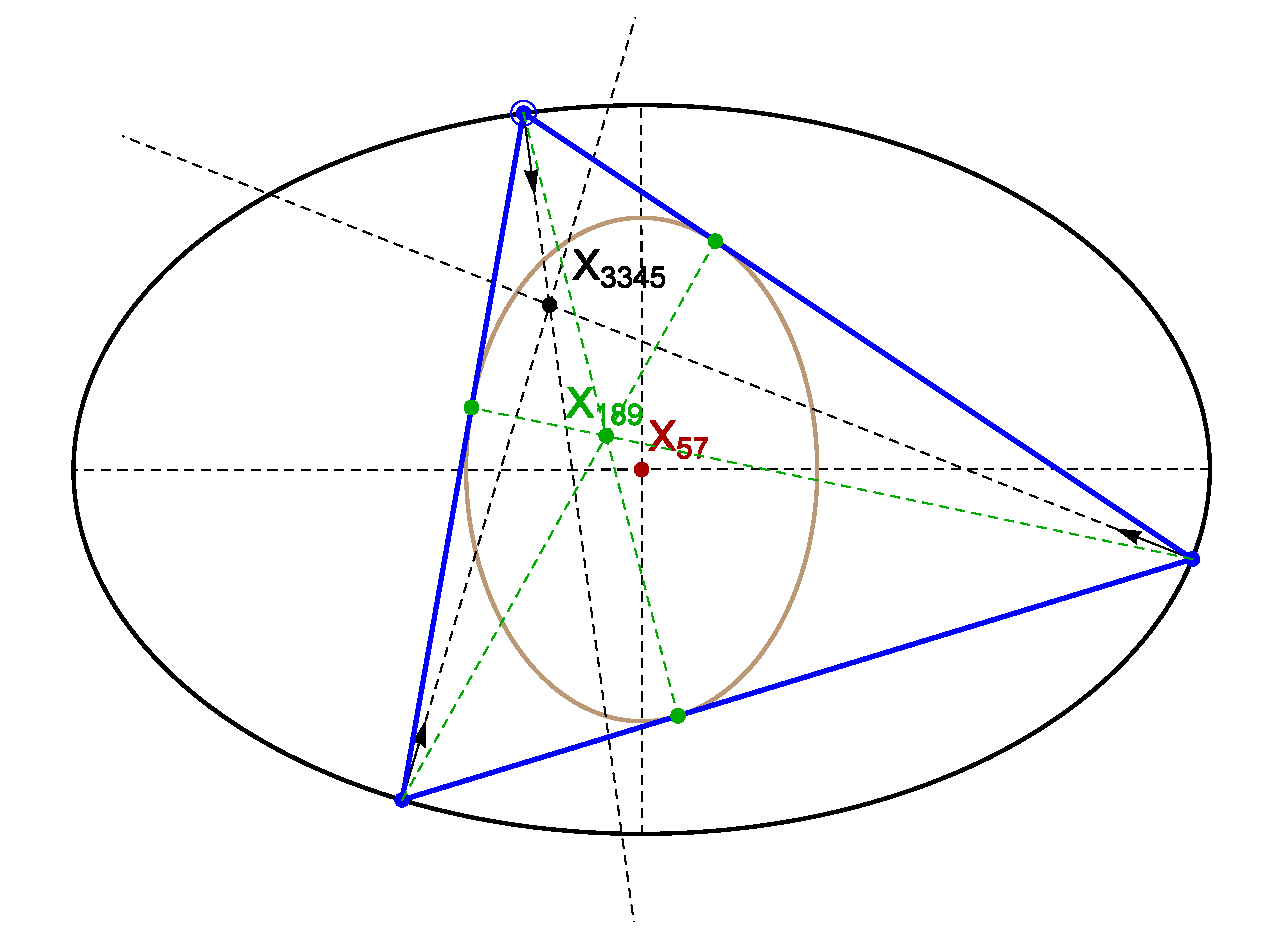
\includegraphics[width=.6\textwidth]{pics_03_310_poncelet_x57.eps}
%    \caption{A Poncelet 3-periodic (blue) interscribed between the $X_{57}$-centered circumconic and inconic. $X_{189}$ is the inconic's Brianchon point. Normals at the circumconic vertices concur at $X_{3345}$. $X_{57}$ remains stationary over the family. \href{https://youtu.be/QQSN\_ndDJQk}{Video}}
%    \label{fig:03-x57}
%\end{figure}

\begin{figure}
    \centering
    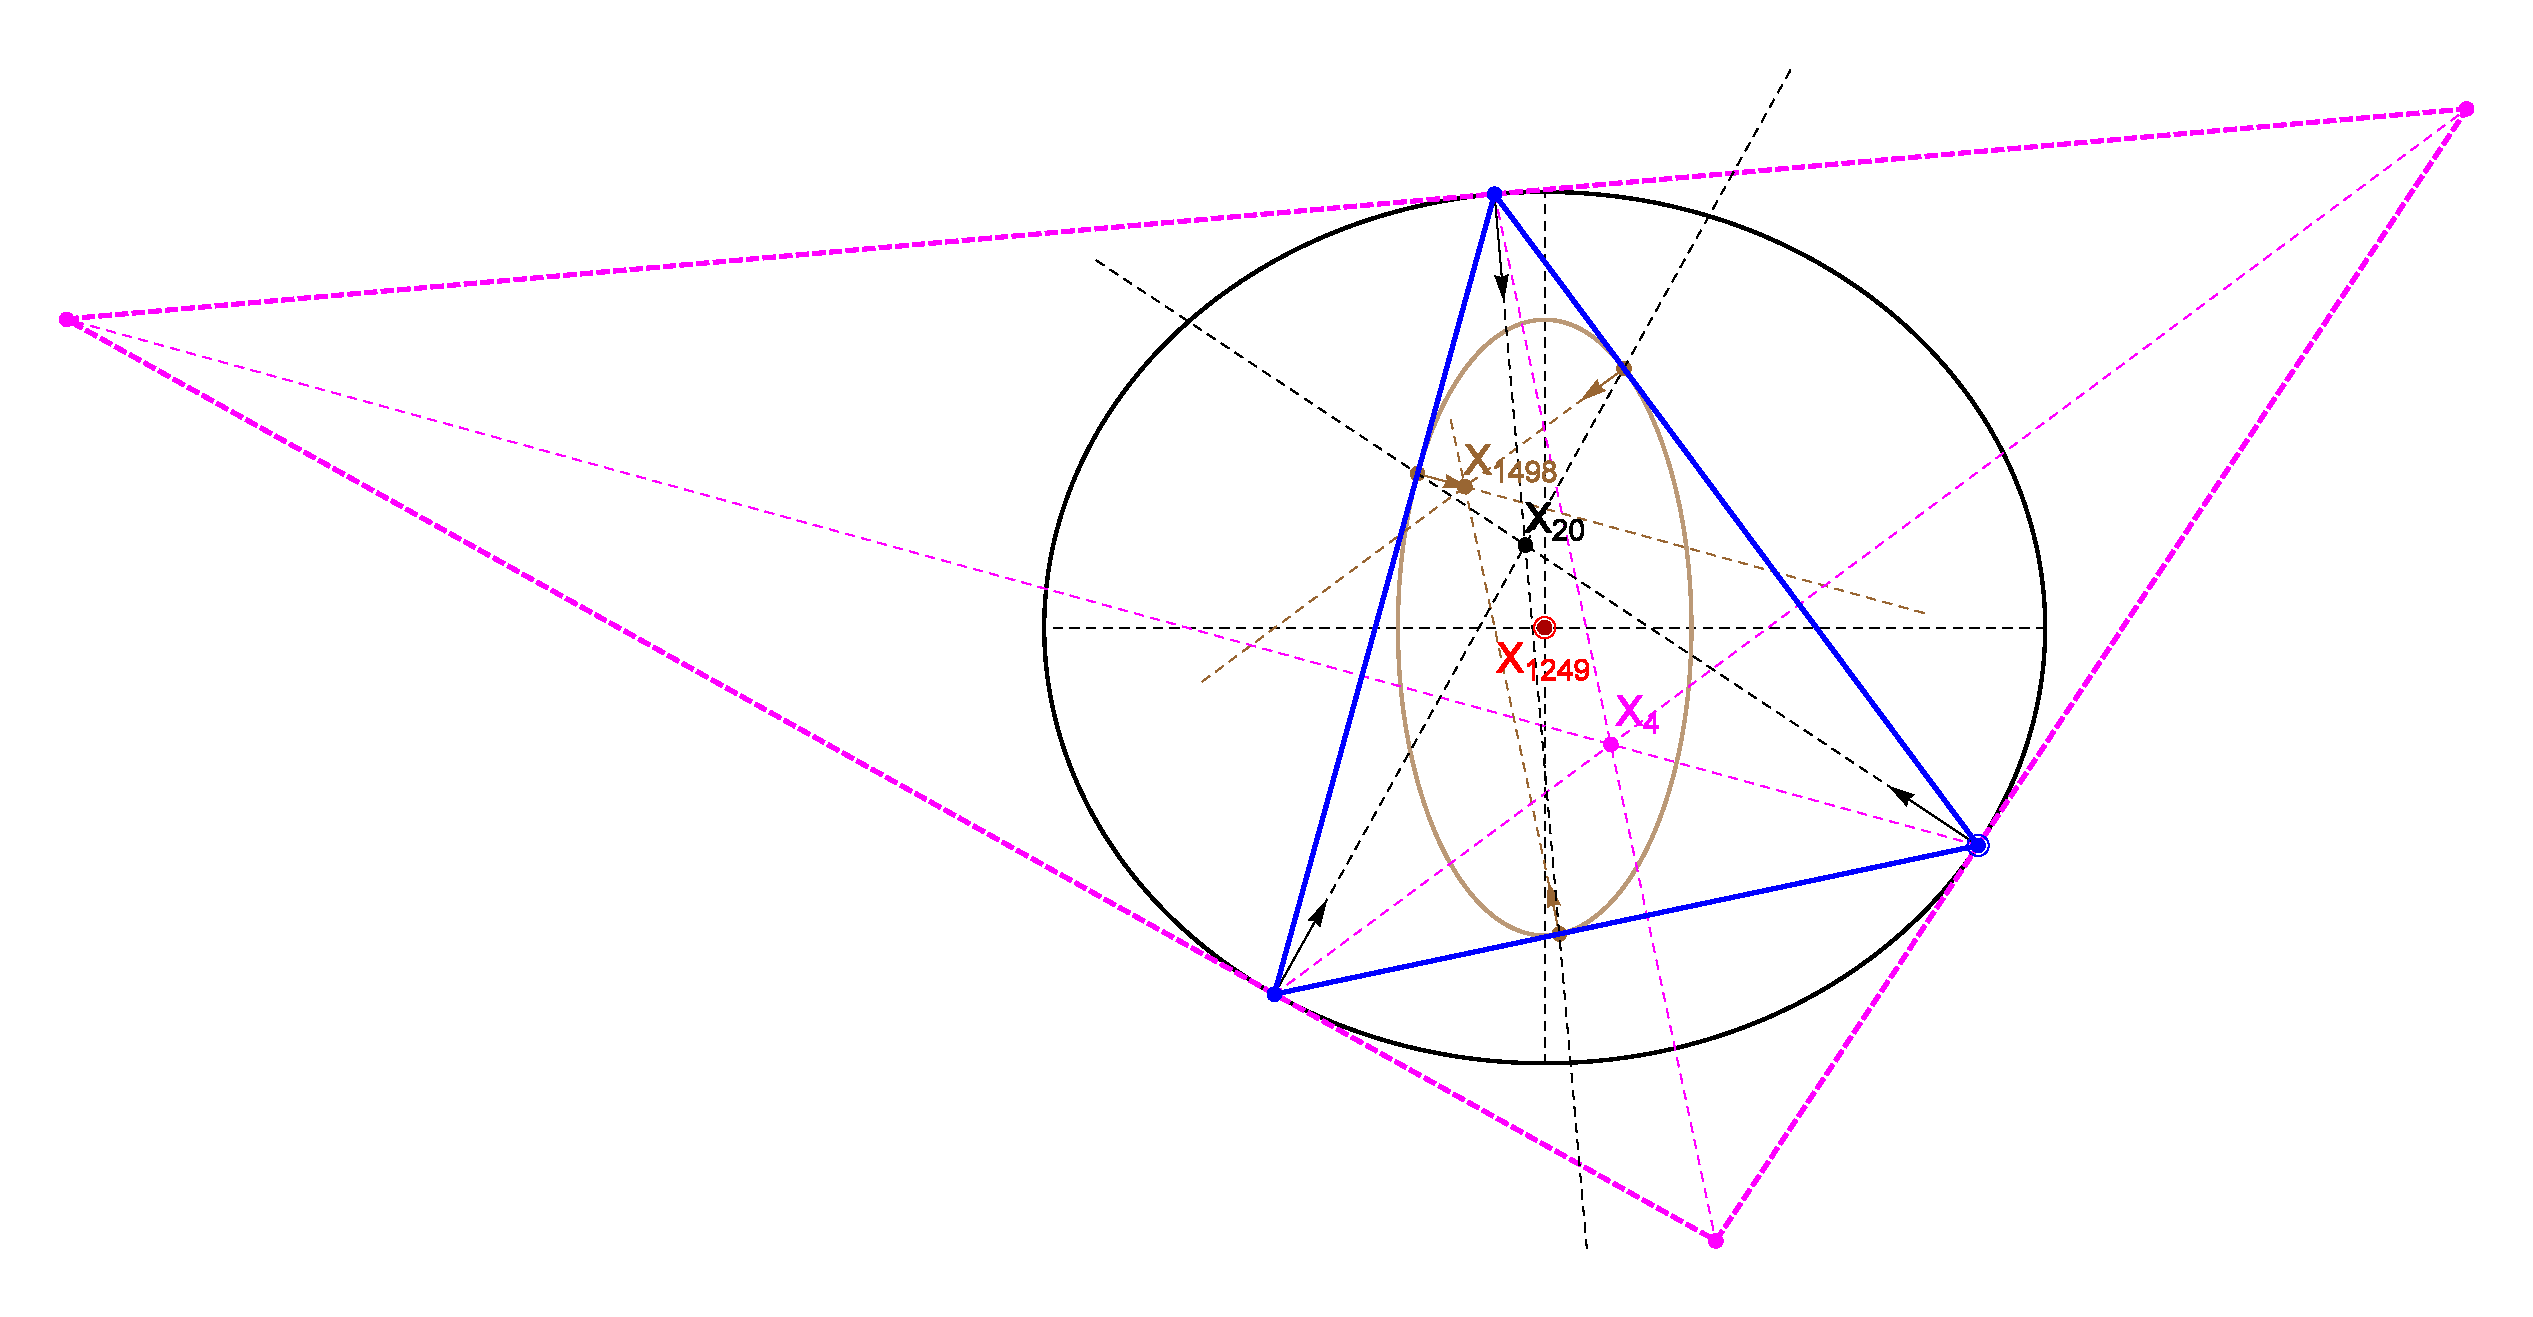
\includegraphics[width=\textwidth]{pics_03_315_poncelet_x1249.eps}
    \caption{A Poncelet 3-periodic (blue) interscribed between the $X_{1249}$-centered circumconic $\Cm$ (black) and inconic $\I$ (brown); over the family, said center remains stationary. Since the center lies on the Thomson cubic, (i) $\Cm$ and $\I$ are axis-parallel, (ii) the normals to $\Cm$ at the vertices concur (at $X_{20}$ in this case), and (iii) the normals to $\I$ at the contact points also concur (at $X_{1498}$). It turns out $X_{20}$ doubles up as the Brianchon point of $\I$, and $X_4$ is the perspector of $\Cm$, i.e., the perspector of its polar triangle (magenta) with respect to $\Cm$. \href{https://youtu.be/QQSN\_ndDJQk}{Video}}
    \label{fig:03-x1249}
\end{figure}

\begin{question}
Given a triangle, compute its $X_7$-centered inconic and circumconic. Prove that 3-periodics interscribed in said conics will not maintain $X_7$ stationary. Prove the same by taking the conic pair's center to be $X_8$ and $X_{10}$, i.e., in neither of these cases will the original center remain stationary. Report the Brianchon point for all said inconics.
\label{que:03-x7}
\end{question}

%\begin{table}
%\centering
%\begin{tabular}{|r|c|c|c|c|c|c|c|}
%\hline
%\makecell[rc]{Poncelet\\family} &
%center &
%\makecell[cc]{norms.\\concur} &
%\makecell[cc]{concur\\ \texttt{bit.ly/*}} & 
%inconic & 
%\makecell[cc]{Brian-\\chon} &
%\makecell[cc]{caustic\\contact tri} &
%\makecell[cc]{contact tri\\ \texttt{bit.ly/*}} \\
%\hline
%incircle & $X_1$ & $X_{84}$ & \href{https://bit.ly/3eVuCQY&}{\texttt{3eVuCQY}} &  %incircle & $X_7$ & intouch & \href{https://bit.ly/3tYYu3h}{\texttt{3tYYu3h}}\\
%homothetic & $X_2$ & $X_4$ & \href{https://bit.ly/3eXSRhC}{\texttt{3eXSRhC}} & %Steiner & $X_2$ & medial & \href{https://bit.ly/3474753}{\texttt{3474753}} \\
%circumcircle & $X_3$ & $X_3$ & \href{https://bit.ly/2RqMqul}{\texttt{2RqMqul}} & ? & %$X_{69}$ & $X_{69}$-cev. & \href{https://bit.ly/2T3qu9f}{\texttt{2T3qu9f}}\\
%dual & $X_4$ & $X_{3346}$ & n/a & ? & $X_{253}$ & $X_{253}$-cev. & %\href{https://bit.ly/2SUfomB}{\texttt{2SUfomB}} \\
%excentral & $X_6$ & $X_{64}$ & \href{https://bit.ly/3hwCTfN}{\texttt{3hwCTfN}} & %orthic & $X_4$ & orthic & \href{https://bit.ly/3uXXI7H}{\texttt{3uXXI7H}}\\
%confocal & $X_9$ & $X_1$ & \href{https://bit.ly/3uTvqLI}{\texttt{3uTvqLI}} & Mandart %& $X_8$ & extouch & \href{https://bit.ly/3wiBeyv}{\texttt{3wiBeyv}} \\
%\hline
%x57 & $X_{57}$ & $X_{3345}$ & n/a & ? & $X_{189}$ &  $X_{189}$-cev. & n/a\\
%\hline
%\end{tabular}
%\caption{Ellipse normal concurrence for various Poncelet families / circumconics.}
%\label{tab:03-normal-concurrence}
%\end{table}

\begin{question}
Prove \cref{prop:03-circum-caustic-curvs}.
\label{que:03-circum-caustic-curvs}
\end{question}
